\documentclass[]{article}
\usepackage{lmodern}
\usepackage{amssymb,amsmath}
\usepackage{ifxetex,ifluatex}
\usepackage{fixltx2e} % provides \textsubscript
\ifnum 0\ifxetex 1\fi\ifluatex 1\fi=0 % if pdftex
  \usepackage[T1]{fontenc}
  \usepackage[utf8]{inputenc}
\else % if luatex or xelatex
  \ifxetex
    \usepackage{mathspec}
  \else
    \usepackage{fontspec}
  \fi
  \defaultfontfeatures{Ligatures=TeX,Scale=MatchLowercase}
\fi
% use upquote if available, for straight quotes in verbatim environments
\IfFileExists{upquote.sty}{\usepackage{upquote}}{}
% use microtype if available
\IfFileExists{microtype.sty}{%
\usepackage{microtype}
\UseMicrotypeSet[protrusion]{basicmath} % disable protrusion for tt fonts
}{}
\usepackage[margin=1in]{geometry}
\usepackage{hyperref}
\hypersetup{unicode=true,
            pdftitle={Weather events causing the most damage to the economy \& public health in the US between 1995 and 2011},
            pdfauthor={Guido van Kleef},
            pdfborder={0 0 0},
            breaklinks=true}
\urlstyle{same}  % don't use monospace font for urls
\usepackage{color}
\usepackage{fancyvrb}
\newcommand{\VerbBar}{|}
\newcommand{\VERB}{\Verb[commandchars=\\\{\}]}
\DefineVerbatimEnvironment{Highlighting}{Verbatim}{commandchars=\\\{\}}
% Add ',fontsize=\small' for more characters per line
\usepackage{framed}
\definecolor{shadecolor}{RGB}{248,248,248}
\newenvironment{Shaded}{\begin{snugshade}}{\end{snugshade}}
\newcommand{\KeywordTok}[1]{\textcolor[rgb]{0.13,0.29,0.53}{\textbf{#1}}}
\newcommand{\DataTypeTok}[1]{\textcolor[rgb]{0.13,0.29,0.53}{#1}}
\newcommand{\DecValTok}[1]{\textcolor[rgb]{0.00,0.00,0.81}{#1}}
\newcommand{\BaseNTok}[1]{\textcolor[rgb]{0.00,0.00,0.81}{#1}}
\newcommand{\FloatTok}[1]{\textcolor[rgb]{0.00,0.00,0.81}{#1}}
\newcommand{\ConstantTok}[1]{\textcolor[rgb]{0.00,0.00,0.00}{#1}}
\newcommand{\CharTok}[1]{\textcolor[rgb]{0.31,0.60,0.02}{#1}}
\newcommand{\SpecialCharTok}[1]{\textcolor[rgb]{0.00,0.00,0.00}{#1}}
\newcommand{\StringTok}[1]{\textcolor[rgb]{0.31,0.60,0.02}{#1}}
\newcommand{\VerbatimStringTok}[1]{\textcolor[rgb]{0.31,0.60,0.02}{#1}}
\newcommand{\SpecialStringTok}[1]{\textcolor[rgb]{0.31,0.60,0.02}{#1}}
\newcommand{\ImportTok}[1]{#1}
\newcommand{\CommentTok}[1]{\textcolor[rgb]{0.56,0.35,0.01}{\textit{#1}}}
\newcommand{\DocumentationTok}[1]{\textcolor[rgb]{0.56,0.35,0.01}{\textbf{\textit{#1}}}}
\newcommand{\AnnotationTok}[1]{\textcolor[rgb]{0.56,0.35,0.01}{\textbf{\textit{#1}}}}
\newcommand{\CommentVarTok}[1]{\textcolor[rgb]{0.56,0.35,0.01}{\textbf{\textit{#1}}}}
\newcommand{\OtherTok}[1]{\textcolor[rgb]{0.56,0.35,0.01}{#1}}
\newcommand{\FunctionTok}[1]{\textcolor[rgb]{0.00,0.00,0.00}{#1}}
\newcommand{\VariableTok}[1]{\textcolor[rgb]{0.00,0.00,0.00}{#1}}
\newcommand{\ControlFlowTok}[1]{\textcolor[rgb]{0.13,0.29,0.53}{\textbf{#1}}}
\newcommand{\OperatorTok}[1]{\textcolor[rgb]{0.81,0.36,0.00}{\textbf{#1}}}
\newcommand{\BuiltInTok}[1]{#1}
\newcommand{\ExtensionTok}[1]{#1}
\newcommand{\PreprocessorTok}[1]{\textcolor[rgb]{0.56,0.35,0.01}{\textit{#1}}}
\newcommand{\AttributeTok}[1]{\textcolor[rgb]{0.77,0.63,0.00}{#1}}
\newcommand{\RegionMarkerTok}[1]{#1}
\newcommand{\InformationTok}[1]{\textcolor[rgb]{0.56,0.35,0.01}{\textbf{\textit{#1}}}}
\newcommand{\WarningTok}[1]{\textcolor[rgb]{0.56,0.35,0.01}{\textbf{\textit{#1}}}}
\newcommand{\AlertTok}[1]{\textcolor[rgb]{0.94,0.16,0.16}{#1}}
\newcommand{\ErrorTok}[1]{\textcolor[rgb]{0.64,0.00,0.00}{\textbf{#1}}}
\newcommand{\NormalTok}[1]{#1}
\usepackage{graphicx,grffile}
\makeatletter
\def\maxwidth{\ifdim\Gin@nat@width>\linewidth\linewidth\else\Gin@nat@width\fi}
\def\maxheight{\ifdim\Gin@nat@height>\textheight\textheight\else\Gin@nat@height\fi}
\makeatother
% Scale images if necessary, so that they will not overflow the page
% margins by default, and it is still possible to overwrite the defaults
% using explicit options in \includegraphics[width, height, ...]{}
\setkeys{Gin}{width=\maxwidth,height=\maxheight,keepaspectratio}
\IfFileExists{parskip.sty}{%
\usepackage{parskip}
}{% else
\setlength{\parindent}{0pt}
\setlength{\parskip}{6pt plus 2pt minus 1pt}
}
\setlength{\emergencystretch}{3em}  % prevent overfull lines
\providecommand{\tightlist}{%
  \setlength{\itemsep}{0pt}\setlength{\parskip}{0pt}}
\setcounter{secnumdepth}{0}
% Redefines (sub)paragraphs to behave more like sections
\ifx\paragraph\undefined\else
\let\oldparagraph\paragraph
\renewcommand{\paragraph}[1]{\oldparagraph{#1}\mbox{}}
\fi
\ifx\subparagraph\undefined\else
\let\oldsubparagraph\subparagraph
\renewcommand{\subparagraph}[1]{\oldsubparagraph{#1}\mbox{}}
\fi

%%% Use protect on footnotes to avoid problems with footnotes in titles
\let\rmarkdownfootnote\footnote%
\def\footnote{\protect\rmarkdownfootnote}

%%% Change title format to be more compact
\usepackage{titling}

% Create subtitle command for use in maketitle
\providecommand{\subtitle}[1]{
  \posttitle{
    \begin{center}\large#1\end{center}
    }
}

\setlength{\droptitle}{-2em}

  \title{Weather events causing the most damage to the economy \& public health
in the US between 1995 and 2011}
    \pretitle{\vspace{\droptitle}\centering\huge}
  \posttitle{\par}
    \author{Guido van Kleef}
    \preauthor{\centering\large\emph}
  \postauthor{\par}
      \predate{\centering\large\emph}
  \postdate{\par}
    \date{13 june 2019}


\begin{document}
\maketitle

\subsection{Synopsis}\label{synopsis}

In this report we aim to find which weather events are the most harmful
to the public health and economy in the United States between the years
1995 and 2011. We obtained data from the National Climatic Data Center
(NCDC) who receive the storm related data from the National Weather
Service (NWS). We specifically obtained data between the years 1995 and
2011 since there are more recent measurements and we are especailly
interested in recents \& recurring events, because these are more
predictable and it's easier to come up with policies to reduce the
health \& economical damage caused by these events. From these data, we
found that, Tornado's are by far the most harmful to both the publich
health and economy. However, on average extreme heat is doing more
damage to public health per incident and hurricanes are on average doing
more damage to the economy, but these events are occuring less often
than Tornado's so the overall impact is lower.

\subsection{Data Processing}\label{data-processing}

\subsubsection{Download \& read data}\label{download-read-data}

\begin{enumerate}
\def\labelenumi{\arabic{enumi}.}
\tightlist
\item
  Load the libraries needed for the analysis
\item
  Download the data to a local directory \& then read it into an R
  object: rawdata.
\end{enumerate}

\begin{Shaded}
\begin{Highlighting}[]
\KeywordTok{library}\NormalTok{(downloader)}
\end{Highlighting}
\end{Shaded}

\begin{verbatim}
## Warning: package 'downloader' was built under R version 3.5.3
\end{verbatim}

\begin{Shaded}
\begin{Highlighting}[]
\KeywordTok{library}\NormalTok{(dplyr)}
\end{Highlighting}
\end{Shaded}

\begin{verbatim}
## Warning: package 'dplyr' was built under R version 3.5.3
\end{verbatim}

\begin{verbatim}
## 
## Attaching package: 'dplyr'
\end{verbatim}

\begin{verbatim}
## The following objects are masked from 'package:stats':
## 
##     filter, lag
\end{verbatim}

\begin{verbatim}
## The following objects are masked from 'package:base':
## 
##     intersect, setdiff, setequal, union
\end{verbatim}

\begin{Shaded}
\begin{Highlighting}[]
\KeywordTok{library}\NormalTok{(ggplot2)}
\end{Highlighting}
\end{Shaded}

\begin{verbatim}
## Warning: package 'ggplot2' was built under R version 3.5.3
\end{verbatim}

\begin{Shaded}
\begin{Highlighting}[]
\KeywordTok{library}\NormalTok{(lubridate)}
\end{Highlighting}
\end{Shaded}

\begin{verbatim}
## Warning: package 'lubridate' was built under R version 3.5.2
\end{verbatim}

\begin{verbatim}
## 
## Attaching package: 'lubridate'
\end{verbatim}

\begin{verbatim}
## The following object is masked from 'package:base':
## 
##     date
\end{verbatim}

\begin{Shaded}
\begin{Highlighting}[]
\KeywordTok{library}\NormalTok{(tidyr)}
\end{Highlighting}
\end{Shaded}

\begin{verbatim}
## Warning: package 'tidyr' was built under R version 3.5.2
\end{verbatim}

\begin{Shaded}
\begin{Highlighting}[]
\ControlFlowTok{if}\NormalTok{(}\OperatorTok{!}\KeywordTok{dir.exists}\NormalTok{(}\StringTok{"./data"}\NormalTok{))\{}\KeywordTok{dir.create}\NormalTok{(}\StringTok{"./data"}\NormalTok{)\}}
\NormalTok{url <-}\StringTok{ "https://d396qusza40orc.cloudfront.net/repdata%2Fdata%2FStormData.csv.bz2"}
\ControlFlowTok{if}\NormalTok{(}\OperatorTok{!}\KeywordTok{file.exists}\NormalTok{(}\StringTok{"./data/stormdata.csv.bz2"}\NormalTok{))\{}\KeywordTok{download.file}\NormalTok{(url, }\DataTypeTok{destfile =} \StringTok{"./data/stormdata.csv.bz2"}\NormalTok{)\}}
\KeywordTok{unzip}\NormalTok{(}\StringTok{"./data/stormdata.csv.bz2"}\NormalTok{, }\DataTypeTok{exdir =} \StringTok{"./data"}\NormalTok{)}
\end{Highlighting}
\end{Shaded}

\begin{verbatim}
## Warning in unzip("./data/stormdata.csv.bz2", exdir = "./data"): error 1 in
## extracting from zip file
\end{verbatim}

\begin{Shaded}
\begin{Highlighting}[]
\NormalTok{rawdata <-}\StringTok{ }\KeywordTok{read.csv}\NormalTok{(}\StringTok{"./data/stormdata.csv.bz2"}\NormalTok{)}
\end{Highlighting}
\end{Shaded}

\subsubsection{Prepare data}\label{prepare-data}

\begin{enumerate}
\def\labelenumi{\arabic{enumi}.}
\tightlist
\item
  Only selecting data between 1995 and 2011.
\item
  Clean up the rawdata file by removing rows that only contain NA values
\item
  Create columns for the crop and property damage expressed in absolute
  numbers. In the original data file the numbers (PROPDMG and CROPDMG)
  are expressed by the units in the columns (PROPDMGEXP \& CROPDMGEXP).
\end{enumerate}

\begin{Shaded}
\begin{Highlighting}[]
\NormalTok{cleaned_data <-}\StringTok{ }\NormalTok{rawdata }\OperatorTok
\StringTok{        }\KeywordTok{filter}\NormalTok{(}\KeywordTok{as.Date}\NormalTok{(}\KeywordTok{as.character}\NormalTok{(BGN_DATE),}\StringTok{"%d/%m/%Y"}\NormalTok{) }\OperatorTok{>=}\StringTok{ }\KeywordTok{as.Date}\NormalTok{(}\StringTok{"01/01/1995"}\NormalTok{,}\StringTok{"%d/%m/%Y"}\NormalTok{)) }\OperatorTok
\StringTok{        }\KeywordTok{mutate}\NormalTok{(}\DataTypeTok{propdmg =} \KeywordTok{case_when}\NormalTok{(}\KeywordTok{is.na}\NormalTok{(PROPDMG) }\OperatorTok{~}\StringTok{ }\DecValTok{0}\NormalTok{,}
\NormalTok{                                   PROPDMGEXP }\OperatorTok{==}\StringTok{ "K"} \OperatorTok{~}\StringTok{ }\NormalTok{PROPDMG }\OperatorTok{*}\StringTok{ }\DecValTok{1000}\NormalTok{, }
\NormalTok{                                   PROPDMGEXP }\OperatorTok{==}\StringTok{ "M"} \OperatorTok{~}\StringTok{ }\NormalTok{PROPDMG }\OperatorTok{*}\StringTok{ }\DecValTok{1000000}\NormalTok{),}
               \DataTypeTok{cropdmg =} \KeywordTok{case_when}\NormalTok{(CROPDMGEXP }\OperatorTok{==}\StringTok{ "K"} \OperatorTok{~}\StringTok{ }\NormalTok{CROPDMG }\OperatorTok{*}\StringTok{ }\DecValTok{1000}\NormalTok{,}
\NormalTok{                                   CROPDMGEXP }\OperatorTok{==}\StringTok{ "M"} \OperatorTok{~}\StringTok{ }\NormalTok{CROPDMG }\OperatorTok{*}\StringTok{ }\DecValTok{1000000}\NormalTok{,}
                                   \KeywordTok{is.na}\NormalTok{(CROPDMG) }\OperatorTok{~}\StringTok{ }\DecValTok{0}\NormalTok{)) }\OperatorTok
\StringTok{        }\KeywordTok{mutate}\NormalTok{(}\DataTypeTok{propdmg =} \KeywordTok{replace}\NormalTok{(propdmg, }\KeywordTok{is.na}\NormalTok{(propdmg),}\DecValTok{0}\NormalTok{),}
               \DataTypeTok{cropdmg =} \KeywordTok{replace}\NormalTok{(cropdmg, }\KeywordTok{is.na}\NormalTok{(cropdmg),}\DecValTok{0}\NormalTok{)) }\OperatorTok
\StringTok{        }\KeywordTok{filter_all}\NormalTok{(}\KeywordTok{any_vars}\NormalTok{(}\OperatorTok{!}\KeywordTok{is.na}\NormalTok{(.)))}
\end{Highlighting}
\end{Shaded}

\subsection{Results}\label{results}

Top 10 events causing the most fatalities and injuries

\begin{Shaded}
\begin{Highlighting}[]
\NormalTok{agg_victims_tot <-}\StringTok{ }\NormalTok{cleaned_data }\OperatorTok
\StringTok{        }\KeywordTok{group_by}\NormalTok{(EVTYPE) }\OperatorTok
\StringTok{        }\KeywordTok{summarise}\NormalTok{(}\DataTypeTok{fatalities =} \KeywordTok{sum}\NormalTok{(FATALITIES), }
                  \DataTypeTok{injuries =} \KeywordTok{sum}\NormalTok{(INJURIES), }
                  \DataTypeTok{total_victims =} \KeywordTok{sum}\NormalTok{(FATALITIES) }\OperatorTok{+}\StringTok{ }\KeywordTok{sum}\NormalTok{(INJURIES),}
                  \DataTypeTok{avg_victims =} \KeywordTok{mean}\NormalTok{(FATALITIES) }\OperatorTok{+}\StringTok{ }\KeywordTok{mean}\NormalTok{(INJURIES)) }\OperatorTok
\StringTok{        }\KeywordTok{arrange}\NormalTok{(}\KeywordTok{desc}\NormalTok{(total_victims)) }\OperatorTok
\StringTok{        }\KeywordTok{mutate_each}\NormalTok{(}\KeywordTok{funs}\NormalTok{(}\KeywordTok{prettyNum}\NormalTok{(., }\DataTypeTok{big.mark=}\StringTok{","}\NormalTok{)))}
\end{Highlighting}
\end{Shaded}

\begin{verbatim}
## Warning: funs() is soft deprecated as of dplyr 0.8.0
## please use list() instead
## 
## # Before:
## funs(name = f(.)
## 
## # After: 
## list(name = ~f(.))
## This warning is displayed once per session.
\end{verbatim}

\begin{Shaded}
\begin{Highlighting}[]
\NormalTok{top_}\DecValTok{10}\NormalTok{ <-}\StringTok{ }\KeywordTok{head}\NormalTok{(agg_victims_tot,}\DecValTok{10}\NormalTok{)}

\NormalTok{top_10_data <-}\StringTok{ }\NormalTok{cleaned_data }\OperatorTok
\StringTok{        }\KeywordTok{filter}\NormalTok{(EVTYPE }\OperatorTok\StringTok{ }\KeywordTok{unique}\NormalTok{(top_}\DecValTok{10}\OperatorTok{$}\NormalTok{EVTYPE)) }\OperatorTok
\StringTok{        }\KeywordTok{group_by}\NormalTok{(}\DataTypeTok{year =} \KeywordTok{floor_date}\NormalTok{(}\KeywordTok{as.Date}\NormalTok{(}\KeywordTok{as.character}\NormalTok{(BGN_DATE),}\StringTok{"%d/%m/%Y"}\NormalTok{),}\StringTok{"year"}\NormalTok{),}
\NormalTok{                 EVTYPE) }\OperatorTok
\StringTok{        }\KeywordTok{summarise}\NormalTok{(}\DataTypeTok{total_victims =} \KeywordTok{sum}\NormalTok{(FATALITIES) }\OperatorTok{+}\StringTok{ }\KeywordTok{sum}\NormalTok{(INJURIES))}

\KeywordTok{ggplot}\NormalTok{(top_10_data, }\KeywordTok{aes}\NormalTok{(}\DataTypeTok{x =}\NormalTok{ year, }\DataTypeTok{y =}\NormalTok{ total_victims)) }\OperatorTok{+}
\StringTok{        }\KeywordTok{geom_line}\NormalTok{() }\OperatorTok{+}
\StringTok{        }\KeywordTok{facet_wrap}\NormalTok{(.}\OperatorTok{~}\NormalTok{EVTYPE, }\DataTypeTok{scales =} \StringTok{"free"}\NormalTok{) }\OperatorTok{+}
\StringTok{        }\KeywordTok{labs}\NormalTok{(}\DataTypeTok{title =} \StringTok{"Top 10 weather events causing the most victims (injuries & fatalities) in the US since 1995"}\NormalTok{, }\DataTypeTok{x =} \StringTok{"Year"}\NormalTok{, }\DataTypeTok{y =} \StringTok{"Total Victims"}\NormalTok{)}
\end{Highlighting}
\end{Shaded}

\includegraphics{Reproducible_research_-_week_4_-_NOAA_storm_data_analysis_files/figure-latex/top 10 events fatalities \& injuries-1.pdf}

\begin{Shaded}
\begin{Highlighting}[]
\KeywordTok{print}\NormalTok{(}\KeywordTok{head}\NormalTok{(agg_victims_tot,}\DecValTok{10}\NormalTok{))}
\end{Highlighting}
\end{Shaded}

\begin{verbatim}
## # A tibble: 10 x 5
##    EVTYPE            fatalities injuries total_victims avg_victims
##    <chr>             <chr>      <chr>    <chr>         <chr>      
##  1 TORNADO           552        7,991    8,543         0.8907309  
##  2 EXCESSIVE HEAT    967        2,710    3,677         4.630982   
##  3 LIGHTNING         285        1,703    1,988         0.3482221  
##  4 HEAT              739        1,153    1,892         5.821538   
##  5 TSTM WIND         96         1,350    1,446         0.02818768 
##  6 WINTER STORM      100        726      826           0.17463    
##  7 FLASH FLOOD       373        444      817           0.03815617 
##  8 HIGH WIND         97         493      590           0.07375    
##  9 THUNDERSTORM WIND 43         483      526           0.01579153 
## 10 HAIL              2          384      386           0.004407298
\end{verbatim}

Top 10 events causing the most total economical damage

\begin{Shaded}
\begin{Highlighting}[]
\NormalTok{agg_eco_dmg_tot <-}\StringTok{ }\NormalTok{cleaned_data }\OperatorTok
\StringTok{        }\KeywordTok{group_by}\NormalTok{(EVTYPE) }\OperatorTok
\StringTok{        }\KeywordTok{summarise}\NormalTok{(}\DataTypeTok{propdmg_costs =} \KeywordTok{sum}\NormalTok{(propdmg), }
                                 \DataTypeTok{cropdmg_costs =} \KeywordTok{sum}\NormalTok{(cropdmg),}
                                 \DataTypeTok{total_costs =} \KeywordTok{sum}\NormalTok{(propdmg)}\OperatorTok{+}\KeywordTok{sum}\NormalTok{(cropdmg),}
                                 \DataTypeTok{avg_costs =} \KeywordTok{mean}\NormalTok{(propdmg) }\OperatorTok{+}\StringTok{ }\KeywordTok{mean}\NormalTok{(cropdmg)) }\OperatorTok
\StringTok{        }\KeywordTok{arrange}\NormalTok{(}\KeywordTok{desc}\NormalTok{(total_costs)) }\OperatorTok
\StringTok{        }\KeywordTok{mutate_each}\NormalTok{(}\KeywordTok{funs}\NormalTok{(}\KeywordTok{prettyNum}\NormalTok{(., }\DataTypeTok{big.mark=}\StringTok{","}\NormalTok{)))}

\NormalTok{top_}\DecValTok{10}\NormalTok{ <-}\StringTok{ }\KeywordTok{head}\NormalTok{(agg_eco_dmg_tot,}\DecValTok{10}\NormalTok{)}

\NormalTok{top_10_data <-}\StringTok{ }\NormalTok{cleaned_data }\OperatorTok
\StringTok{        }\KeywordTok{filter}\NormalTok{(EVTYPE }\OperatorTok\StringTok{ }\KeywordTok{unique}\NormalTok{(top_}\DecValTok{10}\OperatorTok{$}\NormalTok{EVTYPE)) }\OperatorTok
\StringTok{        }\KeywordTok{group_by}\NormalTok{(}\DataTypeTok{year =} \KeywordTok{floor_date}\NormalTok{(}\KeywordTok{as.Date}\NormalTok{(}\KeywordTok{as.character}\NormalTok{(BGN_DATE),}\StringTok{"%d/%m/%Y"}\NormalTok{),}\StringTok{"year"}\NormalTok{),}
\NormalTok{                 EVTYPE) }\OperatorTok
\StringTok{        }\KeywordTok{summarise}\NormalTok{(}\DataTypeTok{total_costs =} \KeywordTok{sum}\NormalTok{(propdmg)}\OperatorTok{+}\KeywordTok{sum}\NormalTok{(cropdmg))}

\KeywordTok{ggplot}\NormalTok{(top_10_data, }\KeywordTok{aes}\NormalTok{(}\DataTypeTok{x =}\NormalTok{ year, }\DataTypeTok{y =}\NormalTok{ total_costs)) }\OperatorTok{+}
\StringTok{        }\KeywordTok{geom_line}\NormalTok{() }\OperatorTok{+}
\StringTok{        }\KeywordTok{facet_wrap}\NormalTok{(.}\OperatorTok{~}\NormalTok{EVTYPE, }\DataTypeTok{scales =} \StringTok{"free"}\NormalTok{) }\OperatorTok{+}
\StringTok{        }\KeywordTok{labs}\NormalTok{(}\DataTypeTok{title =} \StringTok{"Top 10 weather events causing the most economical damage in the US since 1995"}\NormalTok{, }\DataTypeTok{x =} \StringTok{"Year"}\NormalTok{, }\DataTypeTok{y =} \StringTok{"Total Costs"}\NormalTok{)}
\end{Highlighting}
\end{Shaded}

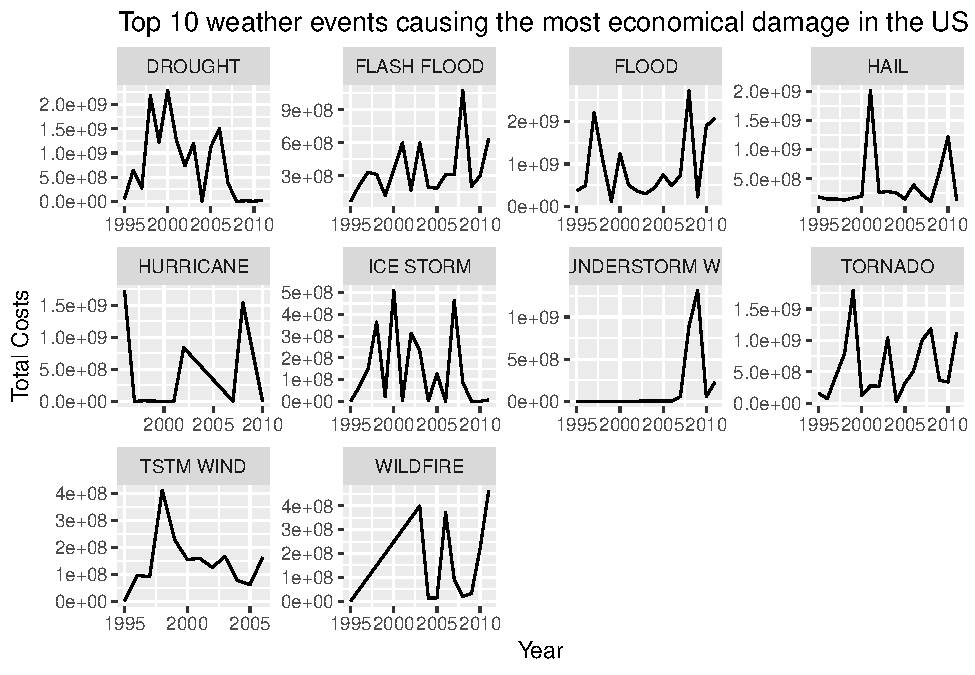
\includegraphics{Reproducible_research_-_week_4_-_NOAA_storm_data_analysis_files/figure-latex/top 10 events economical damage-1.pdf}

\begin{Shaded}
\begin{Highlighting}[]
\KeywordTok{print}\NormalTok{(}\KeywordTok{head}\NormalTok{(agg_eco_dmg_tot,}\DecValTok{10}\NormalTok{))}
\end{Highlighting}
\end{Shaded}

\begin{verbatim}
## # A tibble: 10 x 5
##    EVTYPE            propdmg_costs  cropdmg_costs  total_costs    avg_costs
##    <chr>             <chr>          <chr>          <chr>          <chr>    
##  1 FLOOD             11,536,282,250 4,444,005,500  15,980,287,750 1,447,359
##  2 DROUGHT           1,045,589,000  11,868,301,000 12,913,890,000 5,783,202
##  3 TORNADO           9,693,051,960  151,379,500    9,844,431,460  1,026,424
##  4 HAIL              5,504,376,670  1,170,607,600  6,674,984,270  76,214.11
##  5 FLASH FLOOD       5,409,049,320  593,307,300    6,002,356,620  280,326.8
##  6 HURRICANE         3,334,469,010  791,230,000    4,125,699,010  48,537,6~
##  7 THUNDERSTORM WIND 2,432,066,880  124,773,000    2,556,839,880  76,761.23
##  8 ICE STORM         2,332,991,500  9,830,000      2,342,821,500  2,659,275
##  9 TSTM WIND         1,463,438,360  280,031,900    1,743,470,260  33,986.44
## 10 WILDFIRE          1,399,422,770  228,718,500    1,628,141,270  1,241,908
\end{verbatim}


\end{document}
